% \paragraph{Gender Bias in Wikidata.}
\paragraph{Gender-Based Knowledge Gap: Male vs. Female Representation.}
Gender-based knowledge gap analysis in Wikidata will be performed on 10 Wikidata classes: computer scientist, American singer, American actress/actor, badminton player, businessperson, lawyer, American politician, American writer, American researcher, and American journalist. These classes are chosen to ensure variation in occupations, as gender representation differs across professions. Additionally, six of these classes are limited to American entities to manage scalability, as querying large, global datasets can lead to excessive query time and computational resource constraints. The United States, being a large and well-known country, is expected to provide a broadly reflective sample while keeping the analysis computationally feasible.

To analyze the gap, the first aspect that will be considered is the proportion of each gender in every class. We assumed that there are equal numbers of males and females in real-world and this will be the basis to determine if there is any gap in the data. Pearson's chi-square test (goodness-of-fit) is then performed to test the null and alternative hypotheses with significance level of \(\alpha=\)5\% as follows:

% \(H_0\): The proportions of males and females in a particular class are equal to the real-world proportion

% \(H_1\): The proportions of males and females in a particular class are not equal to the real-world proportion

\begin{table}[h]
    \centering
    \renewcommand{\arraystretch}{1.3}
    \begin{tabular}{|l p{12cm}|} 
        \hline
        \multicolumn{2}{|l|}{\textbf{Gender-Based Knowledge Gap: Entity Count Gap (Pearson's chi-square test)}} \\
        \hline
        \textbf{$H_0$} & The proportions of males and females in a particular class are equal to the assumed real-world proportion of 50\%-50\%. \\
        \textbf{$H_1$} & The proportions of males and females in a particular class are not equal to the assumed real-world proportion of 50\%-50\%. \\
        \hline
        \textbf{Insight 1:} & Across all 10 classes, male entities significantly outnumber female entities in all classes. This suggests a systematic underrepresentation of female entities in Wikidata. \\
        \hline
    \end{tabular}
\end{table}

% \vspace{-3em}

\begin{center}
    \scriptsize
    \makebox[\linewidth]{
    \begin{threeparttable}
    \captionsetup{font=small}
    \caption{Entity Count of 10 Wikidata Classes per Gender Category}
    \label{tab:gender - entity count}
    \begin{tabular}{c | c c c c c | c c} 

    \toprule
        Class Name & Entity & Male & Female & \%Male & \%Female & $\chi^2$ & p-value \\ [0.5ex] 

    \midrule
        American actress/actor & 38655 & 21787 & 16868 & 0.563627 & 0.436373 & 625.96 & 3.78e-138 \\
        American journalist & 18033 & 12402 & 5631 & 0.687739 & 0.312261 & 2542.36 & 0.0 \\
        American politician & 96507 & 85800 & 10707 & 0.889055 & 0.110945 & 58430.57 & 0.0 \\
        American researcher & 5233 & 3634 & 1599 & 0.694439 & 0.305561 & 791.37 & 4.06e-174 \\
        American singer & 16038 & 9198 & 6840 & 0.573513 & 0.426487 & 346.69 & 2.23e-77 \\
        American writer & 33554 & 19656 & 13898 & 0.585802 & 0.414198 & 988.10 & 6.95e-217 \\
        Computer scientist & 19049 & 16180 & 2869 & 0.849388 & 0.150612 & 9301.42 & 0.0 \\
        Badminton player & 25427 & 13493 & 11934 & 0.530656 & 0.469344 & 95.59 & 1.42e-22 \\
        Businessperson & 76758 & 68583 & 8175 & 0.893496 & 0.106504 & 47540.67 & 0.0 \\
        Lawyer & 94479 & 83147 & 11332 & 0.880058 & 0.119942 & 54587.73 & 0.0 \\ [1ex]
    \bottomrule

    \end{tabular}
    \begin{tablenotes}
        \scriptsize
        \item{This table shows the entity count of 10 Wikidata classes per Gender Category. Chi-square test result shows the significance of difference between the entity count of the two genders male and female.}
    \end{tablenotes}
    \end{threeparttable}
    }
\end{center}

From \autoref{tab:gender - entity count}, we can see that there are more male entities than female entities in all of the classes. In terms of entity count, the gender gaps in some classes such as American singer, American actress/actor, badminton player, and American writer, are slim. The gender gaps in some other classes are huge, and it can be observed in the classes of computer scientist, businessperson, lawyer, American politician, journalist, and researcher. This phenomenon can also be easily identified through visualization, as exhibited in \autoref{fig:bias histogram-computer scientist}, where the histogram of the female subclass is much smaller compared to the male. Looking at the chi-square test result, as p-value is well below the chosen significance level, the null hypothesis is rejected in all classes. Hence, we considered the difference of entity count to be significant and conclude that the proportions of males and females in each Wikidata class are not the same as the assumed real-world proportion of 50\%-50\%.

However, it is arguable that, for some classes, the gap in entity count between both genders is expected because, in reality, there are more men than women in the workforce, especially in particular fields such as engineering. As a consequence, it is not reasonable if we expect to have an equal number of males and females entities in Wikidata. Therefore, entity count may not be a good measure of gap because of the nature of the data itself. To address this, we need to evaluate other metrics which can quantify the gap at entity-level.

The next metrics to be considered are the measures of central tendency and dispersion to see where the wealth distribution is concentrated and how the data spread.

\begin{table}[h]
    \centering
    \renewcommand{\arraystretch}{1.3}
    \begin{tabular}{|l p{12cm}|} 
        \hline
        \multicolumn{2}{|l|}{\textbf{Gender-Based Knowledge Gap: Measures of Central Tendency and Dispersion}} \\
        \hline
        \textbf{Insight 1:} & For all 10 classes, female values for mean, median, and mode are generally lower than those of males. Only in the American Singer class does a female (Madonna) appear as the richest individual. \\
        \textbf{Insight 2:} & Positive value of skewness and high value of kurtosis are observed across the board, indicating right-skewed distribution and frequent extreme outliers. \\
        \hline
    \end{tabular}
\end{table}

% \vspace{-3em}

\begin{center}
    \scriptsize
    \makebox[\linewidth]{
    \begin{threeparttable}
    \captionsetup{font=small}
    \caption{Measures of Central Tendency of 10 Wikidata Classes per Gender Category}
    \label{tab:gender - central tendency}
    \begin{tabular}{c | c c c} 

    \toprule
        Class Name & \CellWithForceBreak{Mean \\ (o/m/f)} & \CellWithForceBreak{Median \\ (o/m/f)} & \CellWithForceBreak{Mode \\ (o/m/f)} \\ [0.5ex] 
    \midrule
        American actress/actor & 39.72/40.82/38.31 & 30.00/30.00/28.00 & 19/19/19 \\
        American journalist & 31.30/33.12/27.29 & 24.00/25.00/21.00 & 14/15/14 \\
        American politician & 19.15/19.31/17.90 & 15.00/15.00/15.00 & 9/9/12 \\
        American researcher & 24.24/25.32/21.77 & 20.00/21.00/19.00 & 12/12/15 \\
        American singer & 42.96/43.30/42.51 & 31.00/33.00/30.00 & 18/24/15 \\
        American writer & 39.75/44.05/33.66 & 30.00/33.00/26.00 & 19/21/19 \\
        Computer scientist & 24.30/24.65/22.33 & 19.00/19.00/18.00 & 8/8/11 \\
        Badminton player & 21.90/21.64/22.19 & 16.00/16.00/16.00 & 14/14/14 \\
        Businessperson & 17.06/16.98/17.73 & 13.00/13.00/13.00 & 10/10/9 \\
        Lawyer & 22.58/23.16/18.33 & 19.00/19.00/15.00 & 14/16/12 \\
        [1ex]
    \bottomrule
    \end{tabular}
    \begin{tablenotes}
        \scriptsize
        \item{This table shows the measures of central tendency of 10 Wikidata classes per gender category. Each measure will have 3 values: o (overall), m (male), and f (female).}
    \end{tablenotes}
    \end{threeparttable}
    }
\end{center}

% \vspace{-2em}

\begin{center}
    \scriptsize
    \makebox[\linewidth]{
    \begin{threeparttable}
    \captionsetup{font=small}
    \caption{Measures of Dispersion and Symmetry of 10 Wikidata Classes per Gender Category}
    \label{tab:gender - dispersion and symmetry}
    \begin{tabular}{c | c c c c c} 

    \toprule
        Class Name & \CellWithForceBreak{Min \\ (o/m/f)} & \CellWithForceBreak{Max \\ (o/m/f)} & \CellWithForceBreak{Std. Deviation \\ (o/m/f)} & \CellWithForceBreak{Skewness \\ (o/m/f)} & \CellWithForceBreak{Kurtosis \\ (o/m/f)} \\ [0.5ex] 
    \midrule
        American actress/actor & 4/4/4 & 703/585/703 & 35.15/34.47/35.97 & 4.22/3.65/4.88 & 30.55/22.97/39.11 \\
        American journalist & 4/4/4 & 418/418/363 & 27.78/29.22/23.82 & 4.21/4.17/4.15 & 30.60/29.94/29.09 \\
        American politician & 4/4/4 & 564/564/334 & 15.05/15.07/14.90 & 6.98/7.01/6.83 & 112.45/115.94/84.91 \\
        American researcher & 4/4/4 & 225/225/195 & 17.16/18.46/13.46 & 3.86/3.75/3.74 & 25.74/23.07/31.65 \\
        American singer & 4/5/4 & 703/585/703 & 40.36/36.61/44.90 & 4.15/3.33/4.65 & 29.66/19.78/33.57 \\
        American writer & 4/4/4 & 564/564/435 & 35.82/39.48/28.82 & 3.63/3.37/4.02 & 21.27/18.08/27.34 \\
        Computer scientist & 3/3/3 & 452/452/178 & 19.69/20.35/15.35 & 3.48/3.52/2.25 & 28.77/28.90/9.89 \\
        Badminton player & 9/9/9 & 360/240/360 & 15.98/15.15/16.88 & 4.28/3.94/4.52 & 31.54/23.57/36.62 \\
        Businessperson & 3/3/3 & 585/585/434 & 15.06/14.39/19.81 & 8.07/7.80/8.17 & 142.31/144.95/106.75 \\
        Lawyer & 3/3/3 & 608/608/334 & 17.02/17.34/13.73 & 5.78/5.79/5.67 & 82.87/82.78/78.35 \\[1ex]
    \bottomrule
    \end{tabular}
    \begin{tablenotes}
        \scriptsize
        \item{This table shows the measures of dispersion and symmetry of 10 Wikidata classes per gender category. Each measure will have 3 values: o (overall), m (male), and f (female).}
    \end{tablenotes}
    \end{threeparttable}
    }
\end{center}

From \autoref{tab:gender - central tendency}, female entities generally have lower values of measure of central tendency (mean, median, mode). These characteristics can also be observed from the histogram in \autoref{fig:bias histogram-computer scientist}: female histograms' peak and dense area are located on the left of the male's. However, there are some classes in which the richest entity is a female. An example for this is the class of American Singer, which is shown by \autoref{fig:bias histogram-american singer}. Though the value of mean, median, and mode of count of properties are lower for female compared to male, the richest entity on that class is a female entity \textit{Madonna} (Q1744) with bag of property count of 703, with a significant difference with \textit{Michael Jackson} (Q2831) with bag of property count of 585.

From \autoref{tab:gender - dispersion and symmetry}, we also observed positive values of skewness (skewness > 0) and high kurtosis values (kurtosis > 3) in all classes, denoting the wealth distribution is right-skewed and leptokurtic. The high skewness values indicate that a small number of individuals accumulate disproportionately large property counts. Moreover, high kurtosis values across all genders suggest wealth distributions with heavy tails, meaning that extreme outliers are relatively frequent. Furthermore, we saw higher variability among males, as reflected in their generally wider range of property counts and higher standard deviations. These statistical properties point toward a more unequal wealth distribution among male entities, while females tend to cluster within a lower and more compressed wealth range.

\begin{figure}[!h]
\centering 
\subfloat[Histogram and Marginal Distribution Plot of Wealth for Class Computer Scientist\label{fig:bias histogram-computer scientist}]{%
  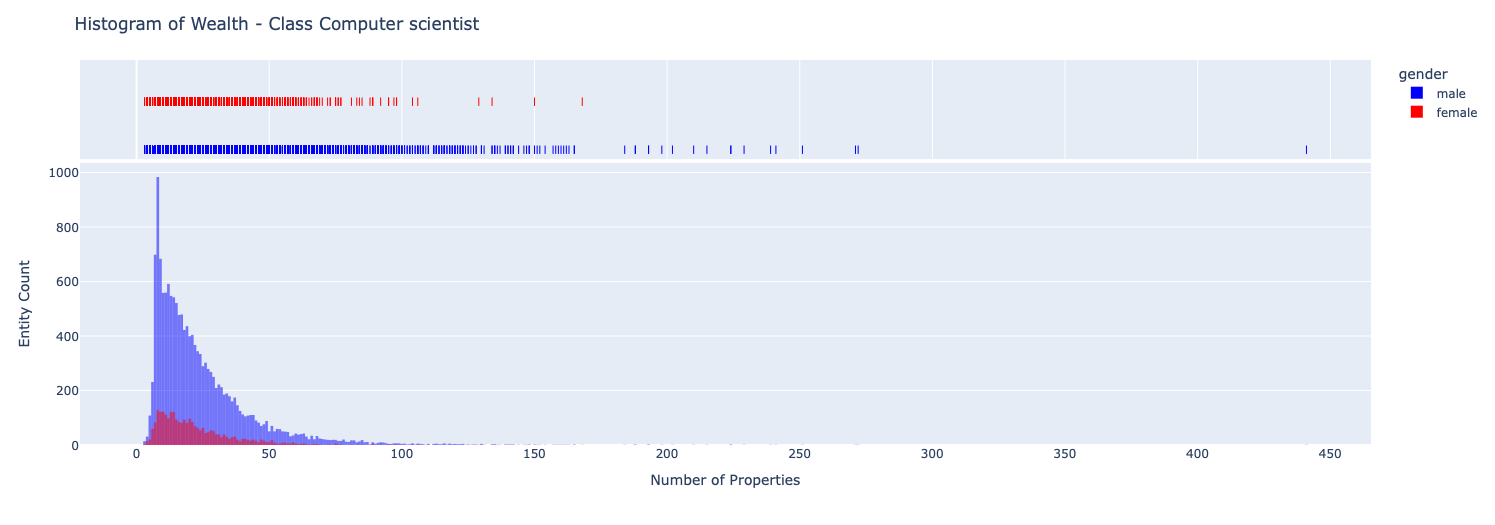
\includegraphics[clip,width=1.0\columnwidth]{Histogram of Wealth - Computer Scientist}%
}

\subfloat[Histogram and Marginal Distribution Plot of Wealth for Class American Singer\label{fig:bias histogram-american singer}]{%
  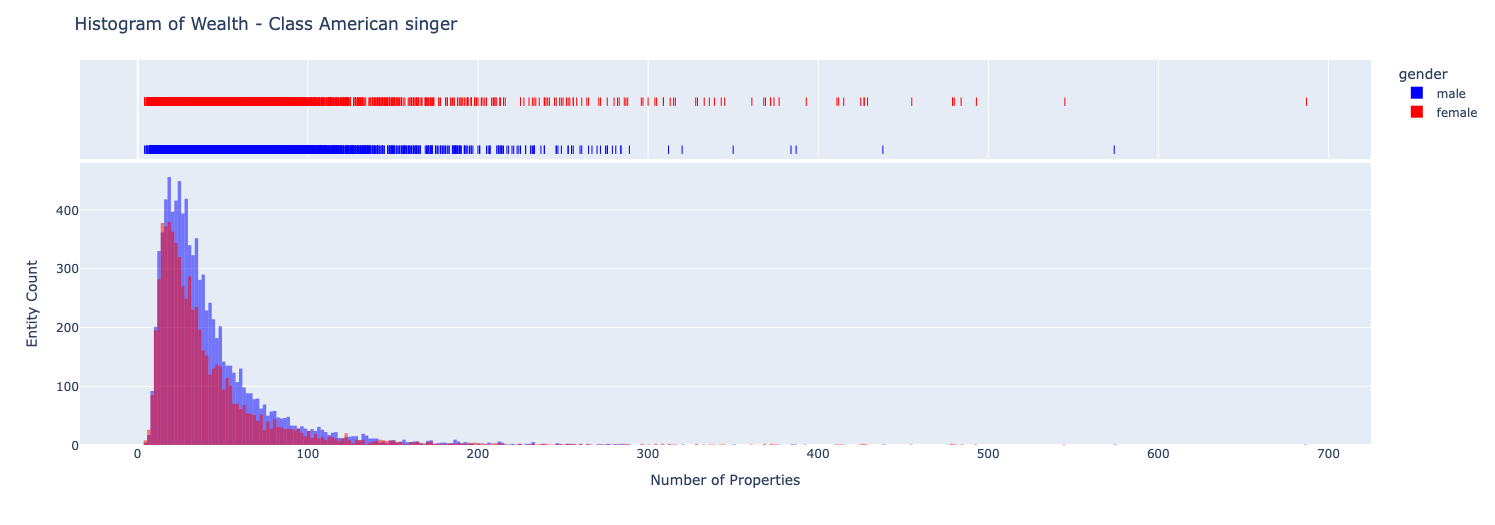
\includegraphics[clip,width=1.0\columnwidth]{Histogram of Wealth - American Singer}%
}

\caption{Histogram of wealth} \label{fig:Histogram of Wealth}

\end{figure}

At a glance we saw female classes are poorer compared to the male classes. To test this, we used t-test and Welch's test. First, we performed F-test to check if the male and female classes have equal variance. The result of F-test is then used to determine the appropiate test to be used in each class. Those with equal variance, i.e., if the p-value is more than 0.05, will use t-test; otherwise Welch's test is used. Then, we performed the appropiate tests to verify the null and alternative hypotheses with significance level of \(\alpha=5\%\) as follows:

% \(H_0\): The means of wealth of males and females in a particular class are equal

% \(H_1\): The means of wealth of males and females in a particular class are not equal

\begin{table}[h!]
    \centering
    \renewcommand{\arraystretch}{1.3}
    \begin{tabular}{|l p{12cm}|} 
        \hline
        \multicolumn{2}{|l|}{\textbf{Gender-Based Knowledge Gap: Mean of Wealth Gap (two-sided t-test and Welch's test)}} \\
        \hline
        \textbf{$H_0$} & The means of wealth of males and females in a particular class are equal. \\
        \textbf{$H_1$} & The means of wealth of males and females in a particular class are not equal. \\
        \hline
        \textbf{Insight 1:} & 9 out of 10 classes shows unequal mean, with 7 of them are in favor of males. \\
        \hline
    \end{tabular}
\end{table}

% \vspace{-3em}

\begin{center}
    \scriptsize
    \makebox[\linewidth]{
    \begin{threeparttable}
    \captionsetup{font=small}
    \caption{F-Test, t-Test, and Welch's Test Result of 10 Wikidata Classes}
    \label{tab:gender - mean test}
    \begin{tabular}{c | c c | c c | c c} 

    \toprule
        Class Name & \CellWithForceBreak{F-Test \\ statistic} & \CellWithForceBreak{F-Test \\ p-value} & \CellWithForceBreak{t-Test \\ statistic} & \CellWithForceBreak{t-Test \\ p-value} & \CellWithForceBreak{Welch's Test \\ statistic} & \CellWithForceBreak{Welch's \\ p-value} \\ [0.5ex] 

    \midrule
        American actress/actor & 0.92 & 0.00 & - & - & 6.93 & 4.27e-12 \\
        American journalist & 1.50 & 1.00 & 13.12 & 4.05e-39 & - & - \\
        American politician & 1.02 & 0.94 & 9.11 & 8.46e-20& - & - \\
        American researcher & 1.88 & 1.00 & 6.92 & 4.91e-12 & - & - \\
        American singer & 0.66 & 0.00 & - & - & 1.19 & 0.23 \\
        American writer & 1.88 & 1.00 & 26.44 & 1.98e-152 & - & - \\
        Computer scientist & 1.76 & 1.00 & 5.83 & 5.80e-09 & - & - \\
        Badminton player & 0.81 & 0.00 & - & - & -2.75 & 0.01 \\
        Businessperson & 0.53 & 0.00 & - & - & -3.34 & 0.00 \\
        Lawyer & 1.60 & 1.00 & 28.47 & 1.69e-177 & - & - \\
    \bottomrule

    \end{tabular}
    \begin{tablenotes}
        \scriptsize
        \item{This table shows the result of F-test, t-test, and Welch's test of 10 Wikidata classes to compare the significance difference between the males and females within each class.}
    \end{tablenotes}
    \end{threeparttable}
    }
\end{center}

Based on F-test on the 10 classes, variance between male and female subclasses was found to be unequal (p < 0.05) in 4 classes, requiring the use of Welch's test. From the test results in \autoref{tab:gender - mean test}, we rejected the null hypothesis in 9 out of 10 class, with the American singer being the only exception with p-value > 0.05. Among them, 7 classes' means are in favor of male. The other 2 classes, badminton player and businessperson, deviate from this trend, where Welch's test results indicate that the female subclasses actually have a higher mean wealth. The extremely small p-values in classes such as American writer and lawyer indicate a very strong statistical signal that the mean wealth differs significantly between genders. Finally, we may conclude that female classes are more likely to have smaller means than male classes, although certain classes may reflect localized or domain-specific representation imbalances. These results reinforce our earlier observations that female entities tend to be poorer in terms of knowledge wealth.

Entity count alone might not be a reliable measure of gap because the nature of the data itself. For instance, in real world, the number of male computer scientists is greater than that of female computer scientists. Therefore, expecting an equal number of male and female entities in Wikidata for this class would be unreasonable. Similarly, measures of central tendency, such as the mean or median, may offer a general overview but fail to capture the distributional nuances of individual entities within a class. To address this, a more holistic metric is needed.

Here, we introduced a new measure: the ratio of top \(x\)\% representation (of male/female) relative to expectation. The value of expectation of a gender in a class is equal to the percentage of that particular in the class. Top \(x\)\% male relative to expectation is the ratio of percentage of male entities in the top \(x\)\% to the expectation. Similarly, top \(x\)\% female relative to expectation is the ratio of percentage of female entities in the top \(x\)\% to the expectation.

\begin{table}[h]
    \centering
    \renewcommand{\arraystretch}{1.3}
    \begin{tabular}{|l p{12cm}|} 
        \hline
        \multicolumn{2}{|l|}{\textbf{Gender-Based Knowledge Gap: Relative Expectation Ratios}} \\
        \hline
        \textbf{Insight 1:} & A ratio value of 1 indicates a balanced distribution, where the group's actual share of wealth aligns with its expected share under equal representation. \\
        \textbf{Insight 2:} & On average across all 8 classes, the bottom six quantiles (i.e., the lower wealth segments) are predominantly composed of female entities, while the top four quantiles (i.e., the wealthier segments) are predominantly male. \\
        \textbf{Insight 3:} & At the individual class level, 6 out of 8 classes show male dominance in the upper wealth quantiles. The exceptions are the businessperson and badminton player classes. \\
        \hline
    \end{tabular}
\end{table}

% \vspace{-2em}

\begin{figure}[!h]
    \centering 
    \subfloat[Ratio of Class Wealth to Expectation per Cumulative Top Percentage - All Classes Average
    \label{fig:test1}]{%
      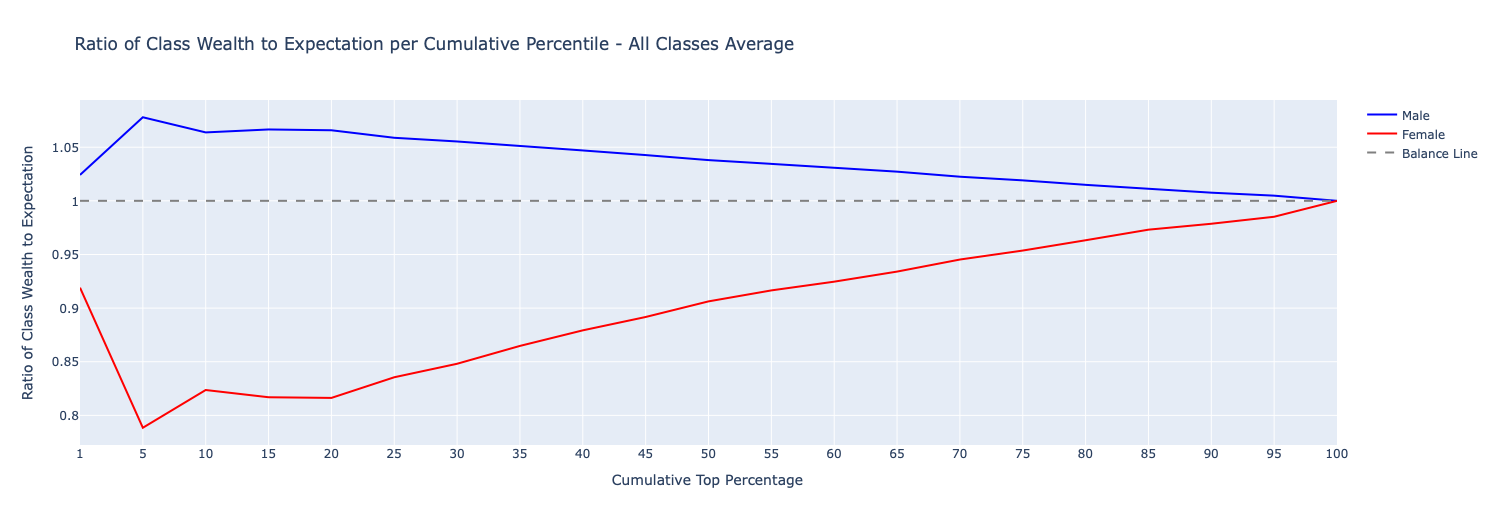
\includegraphics[clip,width=1.0\columnwidth]{Ratio of Class Wealth to Expectation per Cumulative Top Percentage - All Classes Average - Gender}%
    }
    
    \subfloat[Ratio of Class Wealth to Expectation per Quantile - All Classes Average\label{fig:test2}]{%
      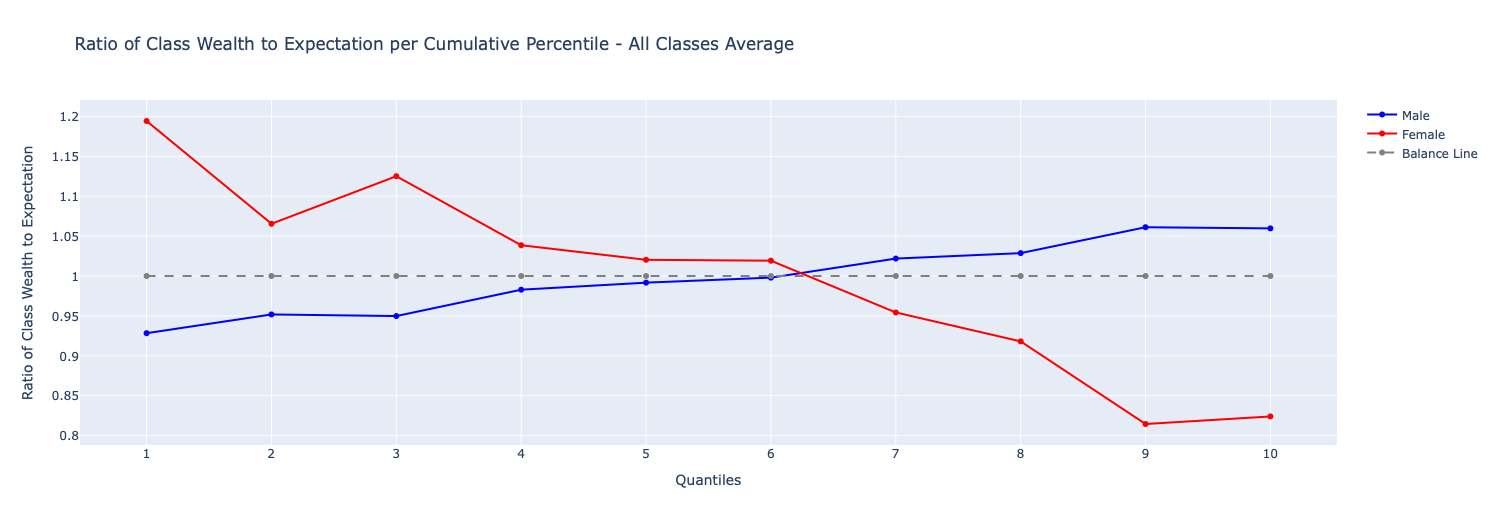
\includegraphics[clip,width=1.0\columnwidth]{Ratio of Class Wealth to Expectation per Quantile - All Classes Average - Gender}%
    }
    
    \caption{Ratio of each gender wealth to expectation} \label{fig:gender - ratio of gender wealth to expectation}
    
\end{figure}

When the shape of distribution of male and female of a class is the same (in other word, the wealth is distributed equivalently to male and female entities), then the value of top \(x\)\% relative to expectation should be 1 for both male and female subclasses. A value higher than 1 indicates domination by that particular gender. Conversely, a value lower than 1 indicates underrepresentation.

From \autoref{fig:gender - ratio of gender wealth to expectation} the value of ratio between top \(x\)\% potion to the expectation in the above tables, we can see that on average, the rich entities are dominated by male. Exceptions are held for 2 classes, that is classes businessperson, and badminton player. In the businessperson class, female dominance in the top quantile (Q10) creates an exception. However, quantiles 2–9 are predominantly male-dominated, albeit only slightly and very close to the balance line. Meanwhile, the lowest quantile (Q1) is significantly female-dominated. The badminton player class deviates from all other classes by exhibiting a distinct zig-zag pattern across quantiles, indicating alternating dominance between males and females, without a clear upward or downward trend.

Moreover, as we set bigger portions (higher percentage), the gap of ratio between the two ender in each class decreases i.e. the value of top \(x\)\% relative to expectation of both genders converge to 1.